\documentclass[tikz, border=5pt]{standalone}
\usepackage{amsmath} % For \binom and \text
\usetikzlibrary{calc} % For coordinate calculations like ($...$)
\usetikzlibrary{decorations.pathreplacing} % For braces

\begin{document}
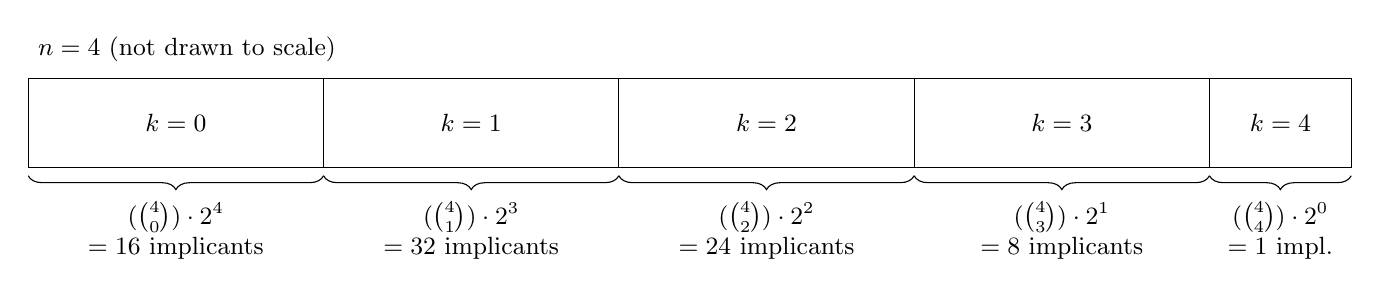
\begin{tikzpicture}[
    every node/.style={font=\small},
    scale=1.5
  ]

% Top labels: "n=4" and the formula on the top right
% The y-coordinate 1.7 provides space above the bar (bar top is at 0.75)
\node[anchor=west] at (0, 1.0) {$n=4$ (not drawn to scale)};


% Define dimensions for the boxes in the bar
\pgfmathsetmacro{\boxheight}{0.75} % Height of the boxes in cm
\pgfmathsetmacro{\ybottom}{0}      % Y-coordinate of the bottom of the boxes
\pgfmathsetmacro{\ytop}{\ybottom + \boxheight} % Y-coordinate of the top of the boxes

% Define widths for each box segment and calculate x-coordinates for division points
% p0 is the starting point of the bar, (0,0)
\coordinate (p0) at (0, \ybottom);
% Widths of the individual boxes
\pgfmathsetmacro{\wzero}{2.5} % Width of K=0 box
\pgfmathsetmacro{\wone}{2.5} % Width of K=1 box
\pgfmathsetmacro{\wtwo}{2.5} % Width of K=2 box
\pgfmathsetmacro{\wthree}{2.5} % Width of K=3 box (narrower)
\pgfmathsetmacro{\wfour}{1.2} % Width of K=4 box (narrower)
% Calculate cumulative x-coordinates for box division lines
\coordinate (p1) at (\wzero, \ybottom);
\coordinate (p2) at (\wzero+\wone, \ybottom);
\coordinate (p3) at (\wzero+\wone+\wtwo, \ybottom);
\coordinate (p4) at (\wzero+\wone+\wtwo+\wthree, \ybottom);
\coordinate (p5) at (\wzero+\wone+\wtwo+\wthree+\wfour, \ybottom); % End point of the last box (total width 9.9cm)

% Draw the outer frame of the entire bar
% ($(p5)+(0,\boxheight)$) calculates the top-right corner of the bar (p5.x, \boxheight)
\draw (p0) rectangle ($(p5)+(0,\boxheight)$);

% Draw internal division lines for the bar segments
% Each line goes from the top of the bar to the bottom at the respective x-coordinate
\draw ($(p1)+(0,\boxheight)$) -- (p1); % Division after K=0
\draw ($(p2)+(0,\boxheight)$) -- (p2); % Division after K=1
\draw ($(p3)+(0,\boxheight)$) -- (p3); % Division after K=2
\draw ($(p4)+(0,\boxheight)$) -- (p4); % Division after K=3

% Place labels "K=i" inside each box segment, centered
% ($(pA)!0.5!(pB)+(0, \boxheight/2)$) calculates the center point of the box between pA and pB
\node at ($(p0)!0.5!(p1)+(0, \boxheight/2)$) {$k=0$};
\node at ($(p1)!0.5!(p2)+(0, \boxheight/2)$) {$k=1$};
\node at ($(p2)!0.5!(p3)+(0, \boxheight/2)$) {$k=2$};
\node at ($(p3)!0.5!(p4)+(0, \boxheight/2)$) {$k=3$};
\node at ($(p4)!0.5!(p5)+(0, \boxheight/2)$) {$k=4$};

% Define settings for the braces and the text below them
\pgfmathsetmacro{\braceoffset}{3pt}   % Gap between the bar and the start of the brace decoration
\pgfmathsetmacro{\braceamplitude}{5pt} % "Height" of the brace curve
\pgfmathsetmacro{\textoffset}{4pt}    % Gap between the end of the brace decoration and the text

% Define a common style for the text nodes below the braces to ensure consistency
\tikzset{formula_text/.style={
    midway, % Place the node at the midpoint of the brace path
    below=\textoffset+\braceamplitude, % Position the node below the brace by a calculated distance
    align=center, % Center-align multi-line text
    anchor=north  % Anchor the text node at its top edge for consistent vertical placement
  }
}

% Create each group (K=0 to K=4) with its brace and mathematical expression

% K=0 group: Brace and text
\draw [decorate, decoration={brace, amplitude=\braceamplitude, mirror, raise=\braceoffset}]
  (p0) -- (p1) node[formula_text] % The brace spans from p0 to p1
  {$(\binom{4}{0}) \cdot 2^4$ \\ $= 16 \text{ implicants}$};

% K=1 group: Brace and text
\draw [decorate, decoration={brace, amplitude=\braceamplitude, mirror, raise=\braceoffset}]
  (p1) -- (p2) node[formula_text] % Brace from p1 to p2
  {$(\binom{4}{1}) \cdot 2^3$ \\ $= 32 \text{ implicants}$};

% K=2 group: Brace and text
\draw [decorate, decoration={brace, amplitude=\braceamplitude, mirror, raise=\braceoffset}]
  (p2) -- (p3) node[formula_text] % Brace from p2 to p3
  {$(\binom{4}{2}) \cdot 2^2$ \\ $= 24 \text{ implicants}$};

% K=3 group: Brace and text
\draw [decorate, decoration={brace, amplitude=\braceamplitude, mirror, raise=\braceoffset}]
  (p3) -- (p4) node[formula_text] % Brace from p3 to p4
  {$(\binom{4}{3}) \cdot 2^1$ \\ $= 8 \text{ implicants}$};

% K=4 group: Brace and text
\draw [decorate, decoration={brace, amplitude=\braceamplitude, mirror, raise=\braceoffset}]
  (p4) -- (p5) node[formula_text] % Brace from p4 to p5
  {$(\binom{4}{4}) \cdot 2^0$ \\ $= 1 \text{ impl.}$};

\end{tikzpicture}
\end{document}
